Avant de dimensionner notre chaîne d'acquisition, nous devons analyser les contraintes qui nous sont imposées.


Tout d'abord, le capteur est un microphone de type piézoélectrique, avec un étage de sortie à transistor intégré, qu'il faut polariser avec une résistance de 2.2k$\Omega$. Le signal en sortie est un signal alternatif de 1mV d'amplitude. Il faut donc amplifier ce signal en le maintenant dans la plage de fonctionnement du dsPIC, c-à-d. entre 0V et 3.3V. Cette plage sera la même pour les ampli-op utilisés ultérieurement.

Ensuite, puisque le signal va être numérisé, il faut ajouter un filtre de garde pour éviter le repliement spectral. Le filtre de garde doit respecter les conditions suivantes : 

\begin{enumerate}
    \item[$\bullet$] Atténuation maximale des fréquences utiles : H1=0.99
    \item[$\bullet$] Atténuation minimale des fréquences repliées : H2=0.05
    \item[$\bullet$] Filtre d'ordre 2 (pour limiter le nombre d'étage de la chaîne analogique)
    \item[$\bullet$] Filtre de Butterworth (réponse la plus plate possible dans la bande passante)
\end{enumerate}

Pour finir, notons que les fréquences utiles sont $900 Hz$ et $1.1 kHz$.

Sachant tout cela, on peut distinguer les tâches suivantes que la chaîne doit réaliser :
\begin{enumerate}
    \item Supprimer la composante continue du signal d'entrée (dûe à la polarisation)
    \item Polariser le signal à 1.65V puisque l'ampli-op est alimenté entre $0V$ et $3V$
    \item Sur base de cette polarisation, amplifier le signal avec un gain de 1650/64.35 dB (le plus tôt possible dans la chaîne pour ne pas amplifier le bruit généré par les composants plus loin dans la chaine)
    \item  Filtrer le signal avant de l'envoyer à l'ADC
\end{enumerate}

Pour nous faciliter le travail, on a décidé de répartir ces tâches en deux blocs. Le premier, qu'on appellera \textbf{amplification}, s'occupe des premières tâches de la chaîne. Ainsi, c'est dans ce bloc qu'on supprimera la composante continue, qu'on polarisera le signal et qu'on l'amplifiera au maximum. Le second bloc sera entièrement réservé au \textbf{filtre de garde}, auquel on pourra éventuellement inclure un gain si nécessaire. On peut rajouter ces deux nouveaux blocs à notre schéma (voir Figure \ref{fig:bloc_chaine}).

\begin{figure}[H]
    \centering
    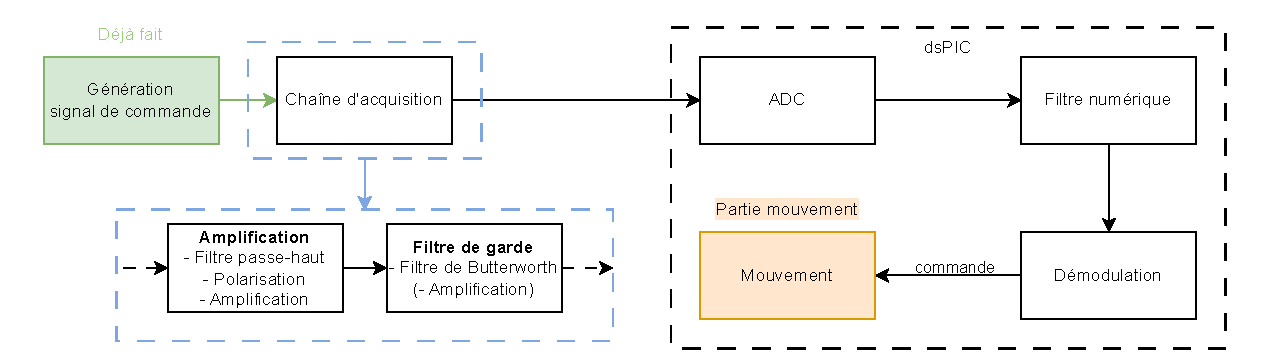
\includegraphics[scale=0.8]{pdffiles/schemabloc.pdf}
    \caption{Schéma-bloc détaillé de la chaîne d'acquisition}
    \label{fig:bloc_chaine}
\end{figure}